% --------------------------------------------------------------------------- %
% --------------------------------------------------------------------------- %
\section{Invisible Z Estimate}
\label{sec:zinv}

The invisible Z background is the dominant SM contribution in many signal regions due to the irreducible nature of the underlying physics. Because the primary interaction produces a massive particle decaying to an invisible final state (\znunu) recoiling against hadronic activity, the signature is fundamentally similar to that of the BSM physics the search is designed to target and difficult to reduce by conventional cuts removing SM background contributions. A robust method leveraging the well-understood Drell-Yan process (\zll) --- an interaction kinematically similar to the invisible Z background --- is used to predict the expected SM contribution based on data while minimizing the reliance on Monte Carlo modeling of the kinematics.

\subsection{Background Prediction}
\label{subsec:zinvPrediction}
The invisible Z background is estimated using dilepton events selected in data. The control region consists of events selected with dilepton triggers, with addition requirements that the leptons are of the same flavor and opposite sign. The momentum of the leading and trailing lepton must also be at least 100\GeV and 30\GeV, respectively, and the invariant mass of the lepton system \mll must be withing 20\GeV of the Z boson mass. The individual CRs are then constructed by removing the dilepton system from the event and applying the baseline preselection requirements as for the signal regions. A detailed description of the CR can be found in section \ref{subsec:zllCR}.

The invisible Z prediction is computed as described by equation \ref{eq:zinvEstimate}, where $N_{\ell\ell}^{\mathrm{CR(SF)}}$ is the number of events in the dilepton same-flavor (SF) region, $N_{\ell\ell}^{\mathrm{CR(OF)}}$ the number of events in the dilepton opposite-flavor (OF) region, $R^{\mathrm{SF/OF}}$ the SF-OF transfer factor, $R_{\mathrm{MC}}^{\znunu / \zll}$ the transfer factor from \zll to \znunu events, and $k(\mttwomath)$ the transfer factor into bins of \mttwo. Each factor is explained in detail below. 
\begin{align}
		N_{\znunu}^{\mathrm{SR}}(\HT,N_\mathrm{j},N_\mathrm{b},\mttwomath) =& \left[ N_{\ell\ell}^{\mathrm{CR(SF)}}(\HT,N_\mathrm{j},N_\mathrm{b}) - N_{\ell\ell}^{\mathrm{CR(OF)}}(\HT,N_\mathrm{j},N_\mathrm{b}) \cdot R^{\mathrm{SF/OF}} \right] \nonumber \\
		& \times R_{\mathrm{MC}}^{\znunu / \zll}(\HT,N_\mathrm{j},N_\mathrm{b}) \cdot k(\mttwomath)
	\label{eq:zinvEstimate}
\end{align}

The second term in equation \ref{eq:zinvEstimate} ($N_{\ell\ell}^{\mathrm{CR(OF)}}\cdot R^{\mathrm{SF/OF}}$) is a correction factor applied to the control region yield to correct for the contribution from processes producing SF and OF event, or {\it flavor-symmetric processes} such as \ttbar production. To compensate for this contribution, a separate control region enriched in \ttbar events is selected from data by using the same selections as the invisible Z CR, except for an inverted selection on the dilepton \pt and \mll requirements. The ratio of \ttbar events is then measured directly from data by counting the yield of SF ($ee$ or $\mu\mu$) and OF ($e\mu$ or $\mu e$) events in this CR. The ratio $R^{\mathrm{SF/OF}}$ is expected to be close to unity based on the underlying physics process, but due to varying acceptance and efficiency effects for different flavor leptons is measured as $R^{\mathrm{SF/OF}} = 1.13 \pm 0.15$, and is stable with respect to event kinematics as shown in figure \ref{fig:rsfof}. The Drell-Yan yield in each control region, as well as the SF yield, OF yield, and transfer factors can be found in tables \ref{tbl:zinvCRs1} and \ref{tbl:zinvCRs2}.
\begin{figure}
	\centering
	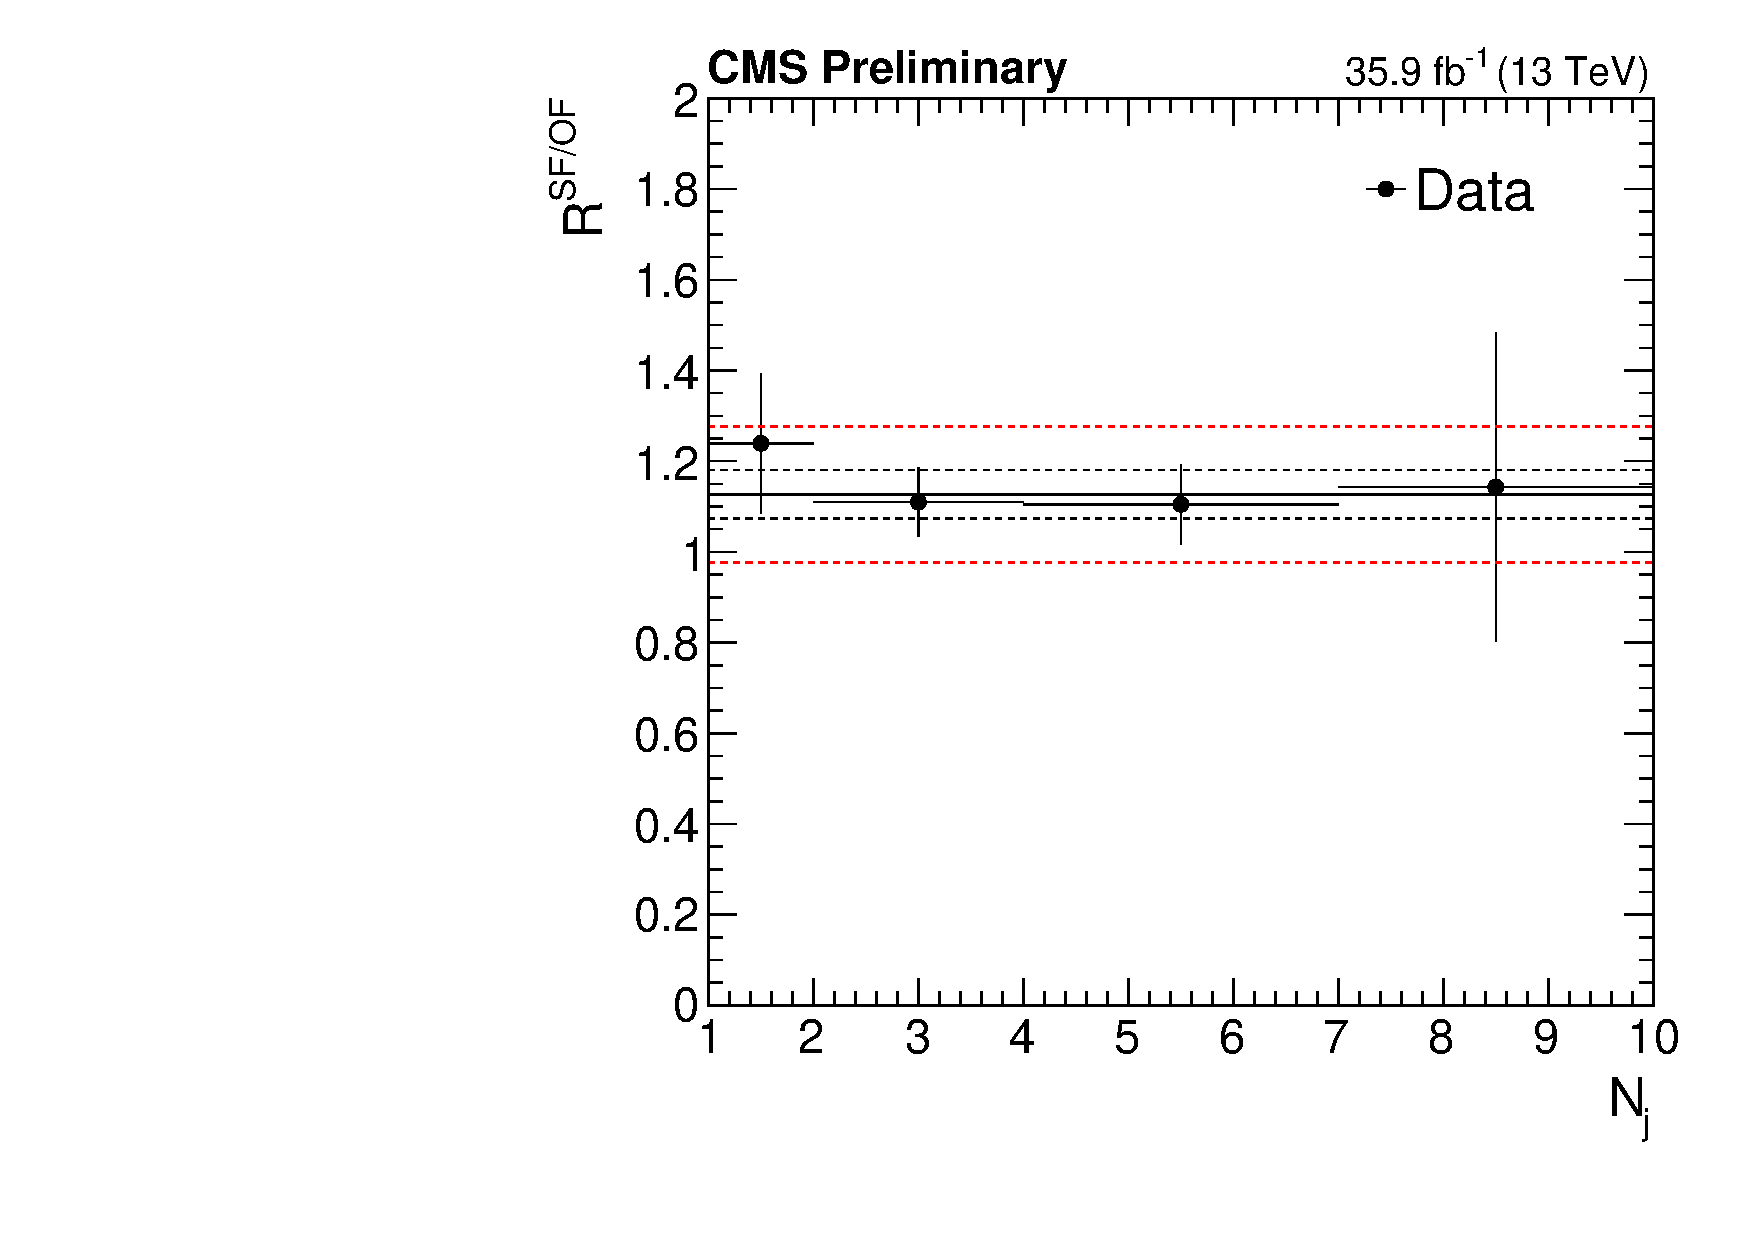
\includegraphics[width=0.48\textwidth]{backgrounds/figs/RSFOF_nj}
	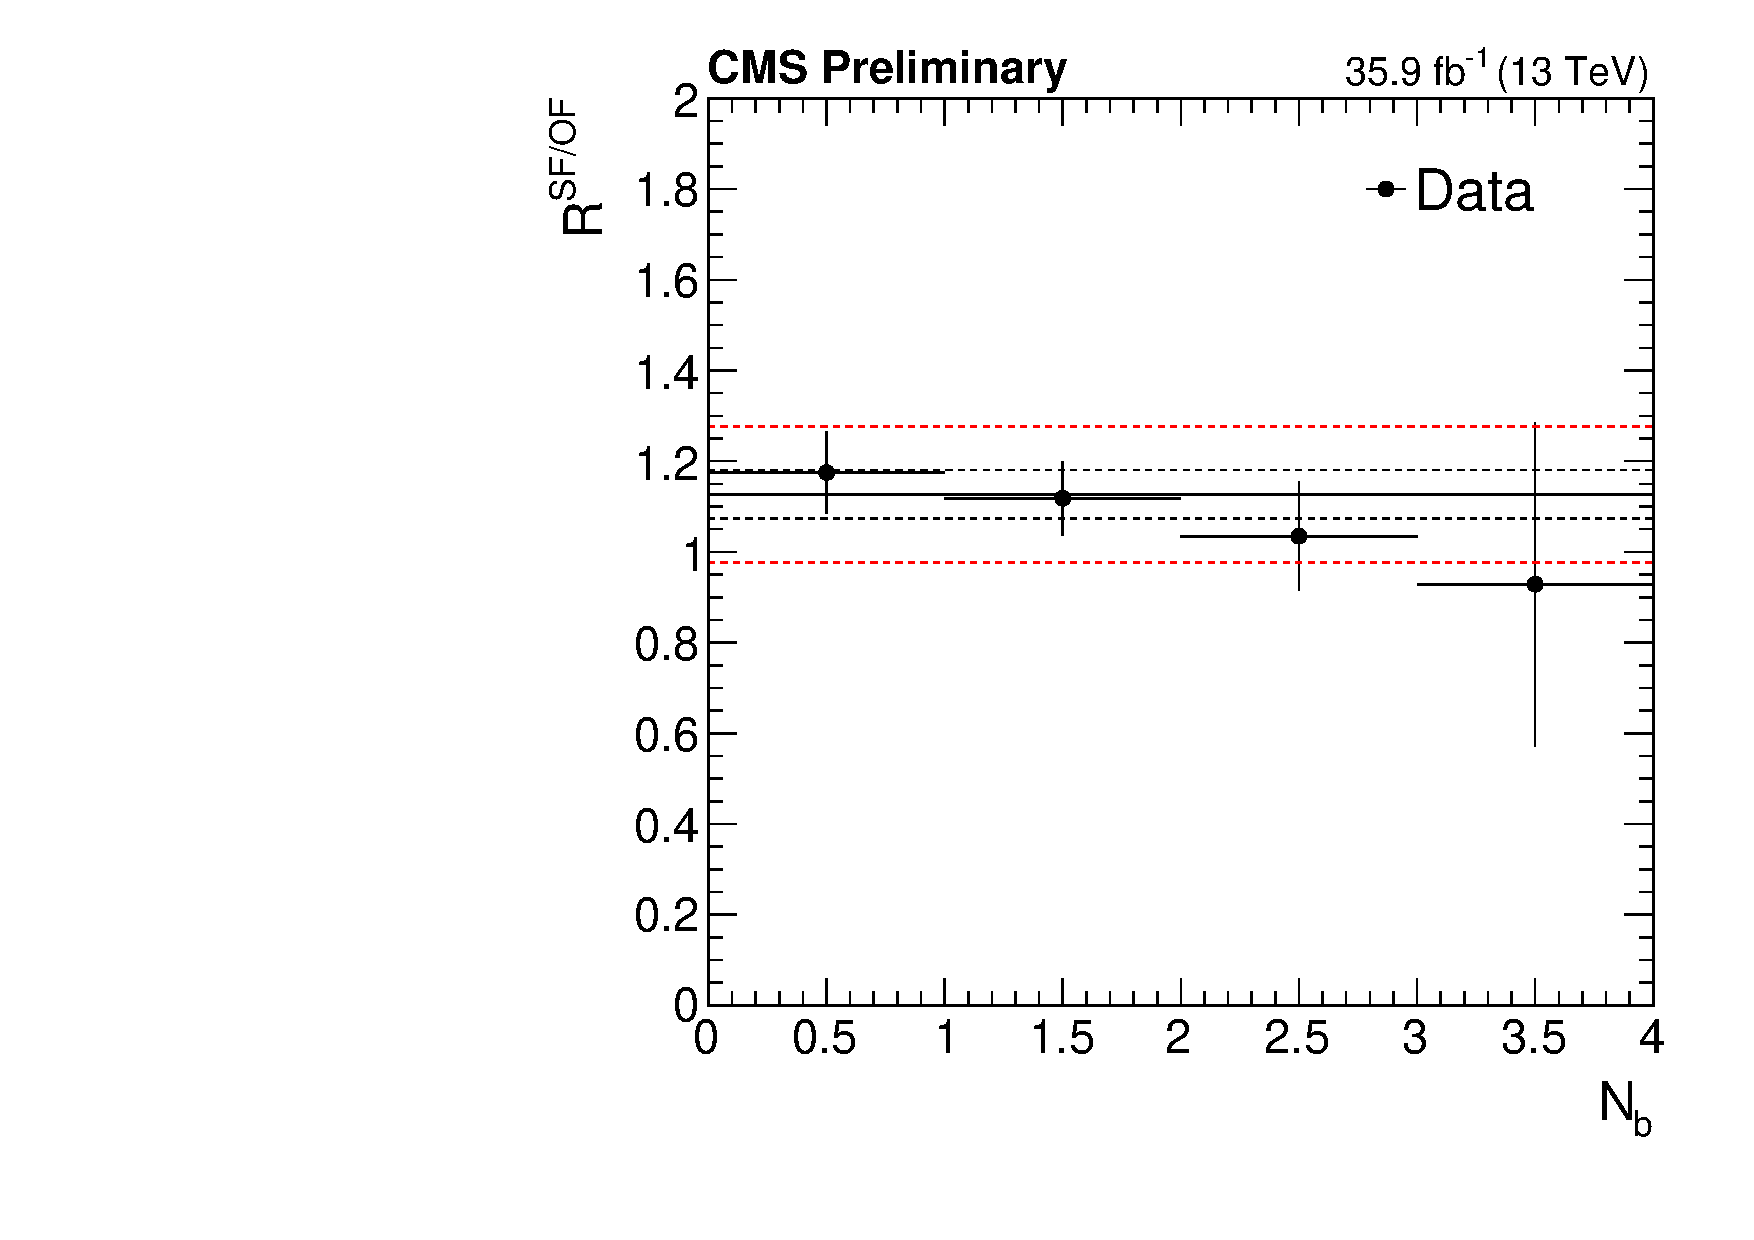
\includegraphics[width=0.48\textwidth]{backgrounds/figs/RSFOF_nb}
	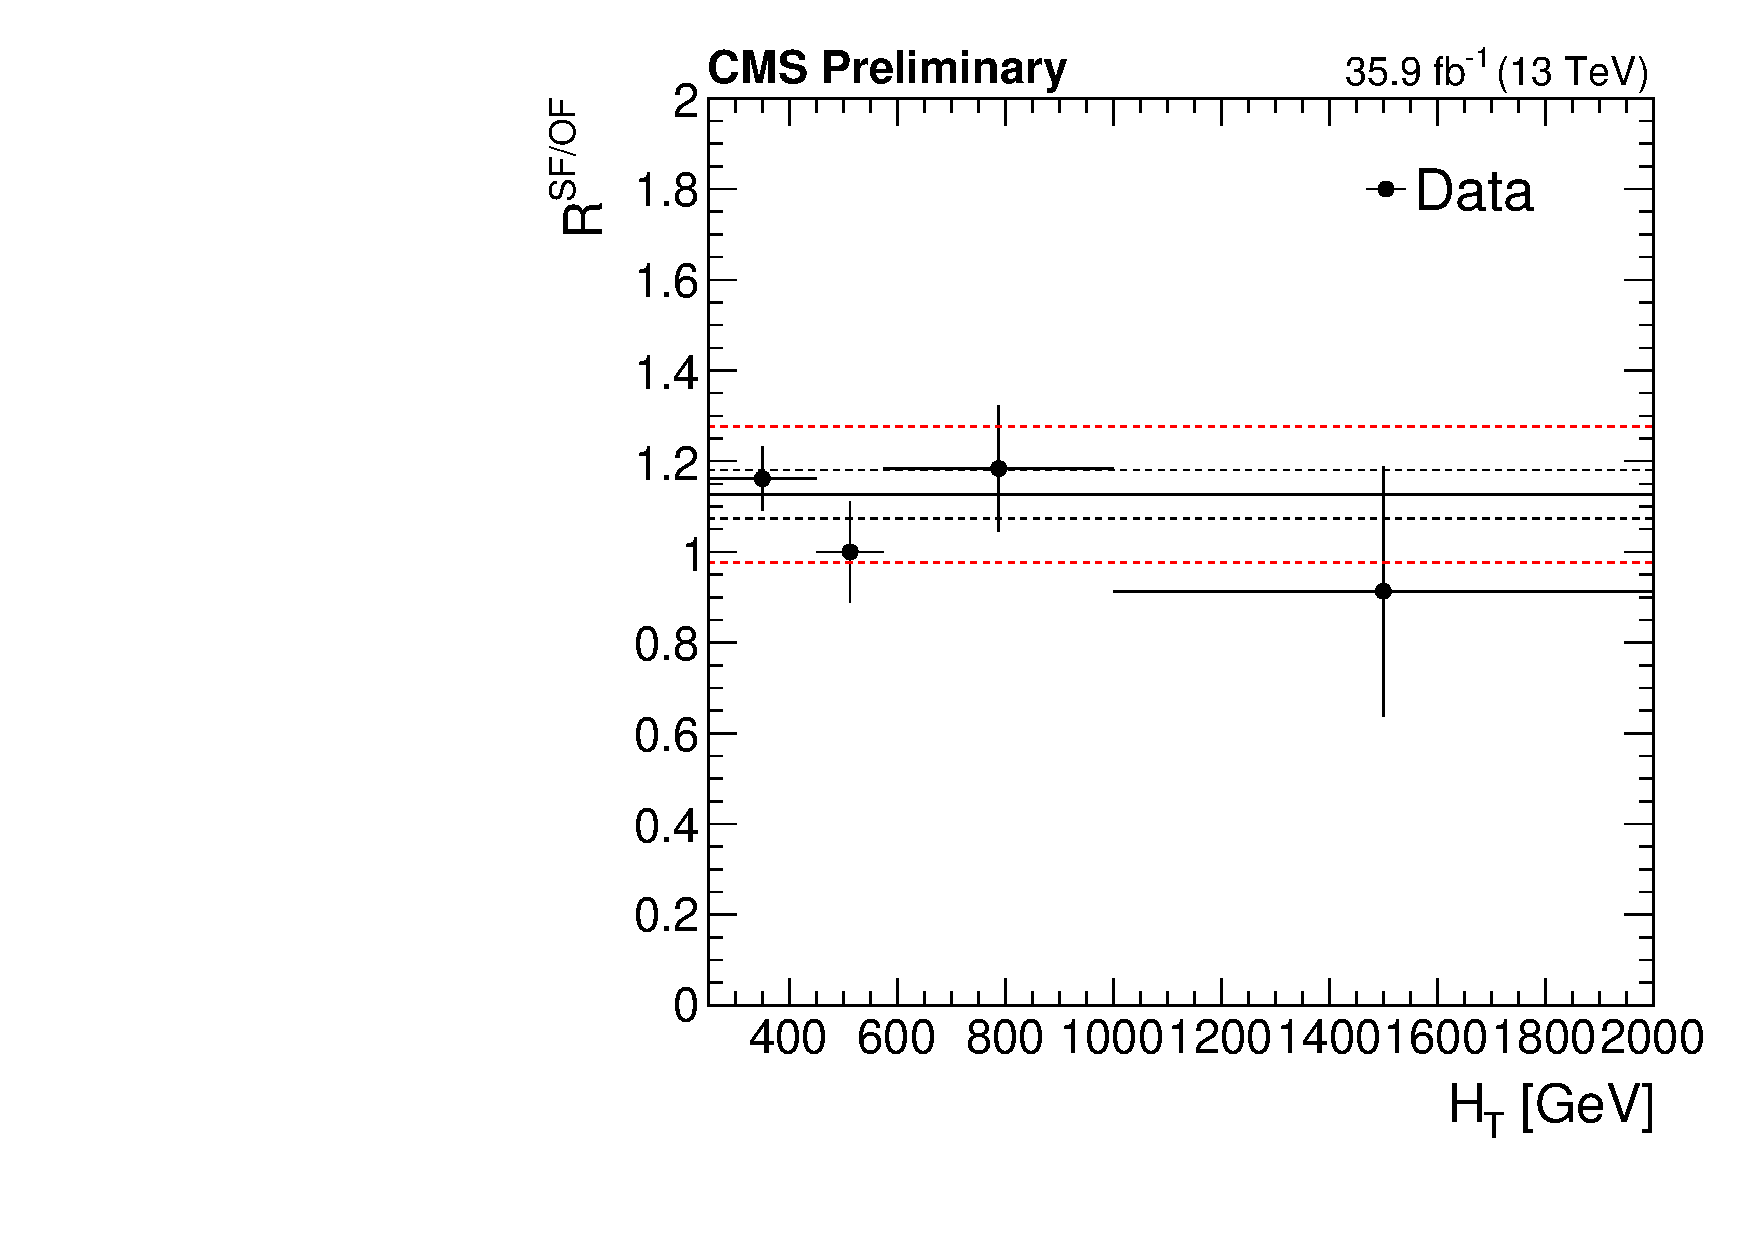
\includegraphics[width=0.48\textwidth]{backgrounds/figs/RSFOF_ht}
	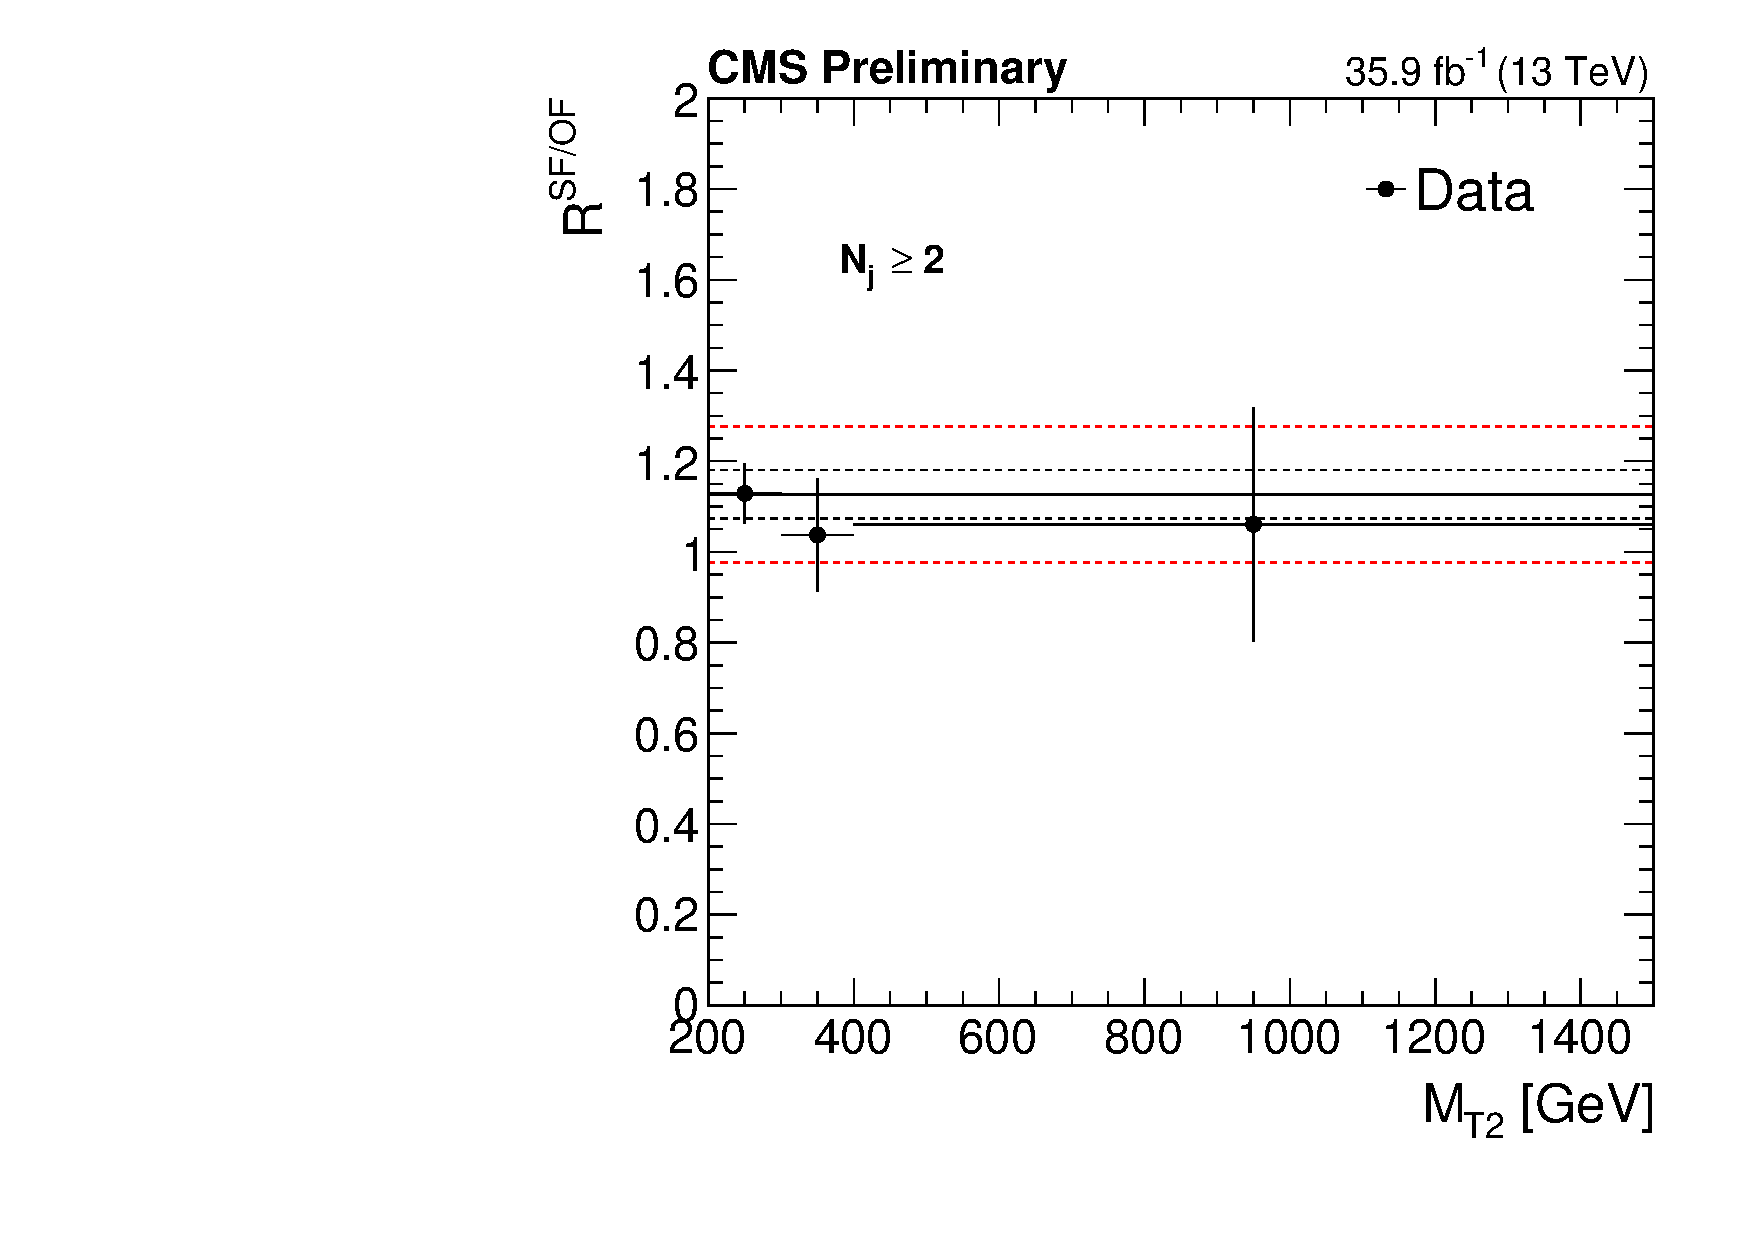
\includegraphics[width=0.48\textwidth]{backgrounds/figs/RSFOF_mt2}
	\renewcommand{\baselinestretch}{1.0}
	\caption[The ratio of same-flavor to opposite-flavor events in a \ttbar enriched control region, as a function of \nj (top left), \nb (top right), \HT (bottom left), and \mttwo (bottom left).]{The ratio of same-flavor to opposite-flavor events in a \ttbar enriched control region, as a function of \nj (top left), \nb (top right), \HT (bottom left), and \mttwo (bottom left). The solid black line corresponds to a constant value of $1.13 \pm 0.15$, while the dashed black lines correspond to the statistical uncertainty and the dashed red lines the total systematic uncertainty.}
	\label{fig:rsfof}
\end{figure}
\begin{table}
	\centering
	\renewcommand{\baselinestretch}{1.0}
	\caption[The control region predicted Drell-Yan (DY) yield, SF yield, OF yield, purity (the rfraction of \zll events), and ratio $R_{\mathrm{MC}}^{\znunu / \zll}$ for the very low, low, and medium \HT topological regions.]{The control region predicted Drell-Yan (DY) yield, SF yield, OF yield, purity (the rfraction of \zll events), and ratio $R_{\mathrm{MC}}^{\znunu / \zll}$ for the very low, low, and medium \HT topological regions. Note that the 7+ jet regions with b-tags (marked with an asterisk) share the same CR, and the fraction of events with different numbers of b-tags is folded into the ratio.}
	\small
	\renewcommand{\arraystretch}{1.0}
	\begin{tabular}{c|c|c|c|c|c|c|c}
\hline \hline
\multicolumn{8}{c}{Invisible Z} \\
\hline
\multicolumn{3}{c|}{Region} & DY Yield & SF Yield & OF Yield & Purity & Ratio\\
$\text{H}_{T}$ [GeV] & $\text{N}_{j}$ & $\text{N}_{b}$ & & & &  \\
\hline
$[250,450]$ &2-3&0&8707.6&8749&37&0.995$\pm$0.001&5.61\\
$[250,450]$ &2-3&1&986.0&1005&17&0.981$\pm$0.004&5.47\\
$[250,450]$ &2-3&2&122.8&125&2&0.982$\pm$0.012&5.31\\
$[250,450]$ &4+&0&1124.5&1129&4&0.996$\pm$0.002&5.88\\
$[250,450]$ &4+&1&215.2&223&7&0.965$\pm$0.012&5.70\\
$[250,450]$ &4+&2&35.9&37&1&0.970$\pm$0.028&5.52\\
$[250,450]$ &2-3&3+&7.0&7&0&1.000$\pm$0.000&6.29\\
$[450,575]$ &2-3&0&1862.7&1875&11&0.993$\pm$0.002&5.08\\
$[450,575]$ &2-3&1&273.2&281&7&0.972$\pm$0.010&4.89\\
$[450,575]$ &2-3&2&19.8&22&2&0.898$\pm$0.064&4.75\\
$[450,575]$ &4-6&0&650.9&661&9&0.985$\pm$0.005&5.49\\
$[450,575]$ &4-6&1&143.4&149&5&0.962$\pm$0.016&5.58\\
$[450,575]$ &4-6&2&27.6&31&3&0.892$\pm$0.056&5.21\\
$[450,575]$ &7+&0&7.0&7&0&1.000$\pm$0.000&5.56\\
$[450,575]$ &7+&1&4.0&4&0&1.000$\pm$0.000&5.18$^{(*)}$\\
$[450,575]$ &7+&2&4.0&4&0&1.000$\pm$0.000&1.87$^{(*)}$\\
$[450,575]$ &2-6&3+&7.0&7&0&1.000$\pm$0.000&5.78\\
$[450,575]$ &7+&3+&4.0&4&0&1.000$\pm$0.000&0.48$^{(*)}$\\
$[575,1000]$ &2-3&0&1347.0&1356&8&0.993$\pm$0.002&4.76\\
$[575,1000]$ &2-3&1&157.3&164&6&0.959$\pm$0.015&4.55\\
$[575,1000]$ &2-3&2&25.8&28&2&0.920$\pm$0.051&4.68\\
$[575,1000]$ &4-6&0&812.4&818&5&0.993$\pm$0.003&5.16\\
$[575,1000]$ &4-6&1&180.0&189&8&0.953$\pm$0.015&5.09\\
$[575,1000]$ &4-6&2&26.3&33&6&0.796$\pm$0.070&5.29\\
$[575,1000]$ &7+&0&32.9&34&1&0.967$\pm$0.031&5.84\\
$[575,1000]$ &7+&1&15.6&19&3&0.823$\pm$0.088&4.41$^{(*)}$\\
$[575,1000]$ &7+&2&15.6&19&3&0.823$\pm$0.088&1.10$^{(*)}$\\
$[575,1000]$ &2-6&3+&5.8&8&2&0.720$\pm$0.159&5.82\\
$[575,1000]$ &7+&3+&15.6&19&3&0.823$\pm$0.088&0.22$^{(*)}$\\
\hline \hline
	\end{tabular}
	\label{tbl:zinvCRs1}
\end{table}

\begin{table}
	\centering
	\renewcommand{\baselinestretch}{1.0}
	\caption[The control region predicted Drell-Yan (DY) yield, SF yield, OF yield, purity (the rfraction of \zll events), and ratio $R_{\mathrm{MC}}^{\znunu / \zll}$ for the high and extreme \HT topological regions.]{The control region predicted Drell-Yan (DY) yield, SF yield, OF yield, purity (the rfraction of \zll events), and ratio $R_{\mathrm{MC}}^{\znunu / \zll}$ for the high and extreme \HT topological regions. Note that the 7+ jet regions with b-tags (marked with an asterisk) share the same CR, and the fraction of events with different numbers of b-tags is folded into the ratio.}
	\small
	\renewcommand{\arraystretch}{1.0}
	\begin{tabular}{c|c|c|c|c|c|c|c}
\hline \hline
\multicolumn{8}{c}{Invisible Z} \\
\hline
\multicolumn{3}{c|}{Region} & DY Yield & SF Yield & OF Yield & Purity & Ratio\\
$\text{H}_{T}$ [GeV] & $\text{N}_{j}$ & $\text{N}_{b}$ & & & &  \\
\hline
$[1000,1500]$ &2-3&0&129.0&129&0&1.000$\pm$0.000&4.76\\
$[1000,1500]$ &2-3&1&25.9&27&1&0.959$\pm$0.038&4.63\\
$[1000,1500]$ &2-3&2&1.9&3&1&0.627$\pm$0.279&4.73\\
$[1000,1500]$ &4-6&0&154.0&154&0&1.000$\pm$0.000&5.10\\
$[1000,1500]$ &4-6&1&42.0&42&0&1.000$\pm$0.000&4.97\\
$[1000,1500]$ &4-6&2&11.0&11&0&1.000$\pm$0.000&5.07\\
$[1000,1500]$ &7+&0&19.0&19&0&1.000$\pm$0.000&5.63\\
$[1000,1500]$ &7+&1&10.0&10&0&1.000$\pm$0.000&4.63$^{(*)}$\\
$[1000,1500]$ &7+&2&10.0&10&0&1.000$\pm$0.000&1.22$^{(*)}$\\
$[1000,1500]$ &2-6&3+&1.0&1&1&1.000$\pm$1.000&4.25\\
$[1000,1500]$ &7+&3+&10.0&10&0&1.000$\pm$0.000&0.20$^{(*)}$\\
$[1500,\infty]$ &2-3&0&29.0&29&0&1.000$\pm$0.000&5.00\\
$[1500,\infty]$ &2-3&1&8.0&8&0&1.000$\pm$0.000&4.66\\
$[1500,\infty]$ &4-6&0&28.9&30&1&0.963$\pm$0.035&5.09\\
$[1500,\infty]$ &4-6&1&14.0&14&0&1.000$\pm$0.000&5.25\\
$[1500,\infty]$ &4-6&2&2.9&4&1&0.720$\pm$0.224&4.80\\
$[1500,\infty]$ &7+&0&5.0&5&0&1.000$\pm$0.000&5.16\\
$[1500,\infty]$ &7+&1&1.9&3&1&0.627$\pm$0.279&3.97$^{(*)}$\\
$[1500,\infty]$ &7+&2&1.9&3&1&0.627$\pm$0.279&1.18$^{(*)}$\\
$[1500,\infty]$ &2-6&3+&1.0&1&0&1.000$\pm$0.000&6.27\\
$[1500,\infty]$ &7+&3+&1.9&3&1&0.627$\pm$0.279&0.18$^{(*)}$\\
\hline \hline
	\end{tabular}
	\label{tbl:zinvCRs2}
\end{table}

The ratio of invisible Z events to Drell-Yan events, $R_{\mathrm{MC}}^{\znunu / \zll}$, is measured in simulation for each CR. The ratio accounts for the branching fraction differences between \zll and \znunu decays, as well as differences in lepton acceptance and efficiency for dilepton pairs in the CR (including corrections for differences in lepton efficiency between data and simulation).

The transfer factor $k(\mttwomath)$ uses a combination of data and simulation information to reduce the dependence of the prediction on the \mttwo shape modeling in simulation. Based on simulation, the \mttwo shape in ever \HT region is independent of \nb. In addition, in the extreme \HT region $\HT > 1500\GeV$, the shape is also independent of \nj. Based on these findings, \mttwo shape templates are constructed for each \HT and \nj region (inclusive in \nb\footnote{The only exception is for regions with more than 2 b-tags (2j3b and 2-6j3b), where at least 3 jets are required so as to avoid biasing the \nj distribution when requiring more b-tags than jets.}), with one single template for the extreme \HT region (which is also inclusive in \nj). 

The \mttwo distribution, $k(\mttwomath)$, for each topological region is constructed from dilepton events in data where statistics allows, and \znunu simulation where statistics are sparse. In each template region, the greatest \mttwo bin is iteratively combined with the next-greatest bin until the total expected SM background yield in simulation is at least 50 events. For uncombined bins (where statistics in data is sufficient), the \mttwo shape is taken directly from dilepton data, corrected for the ratio $R_{\mathrm{MC}}^{\znunu / \zll}$. In the low-statistics combined regime, the \mttwo shape in \znunu simulation is used to determine the fraction of events in each \mttwo bin after normalizing the simulation yield to data in the combined bins. The extrapolation point after which the \mttwo shape is based on simulation in each signal region can be found in tables \ref{tbl:zinvHybridPoint1} and \ref{tbl:zinvHybridPoint2}.
\begin{table}
	\centering
	\renewcommand{\baselinestretch}{1.0}
	\caption[The \mttwo extrapolation point for the very low, low, and medium \HT topological regions, beyond which shape data from simulation is used to extrapolate the invisible Z estimate into \mttwo bins.]{The \mttwo extrapolation point for the very low, low, and medium \HT topological regions, beyond which shape data from simulation is used to extrapolate the invisible Z estimate into \mttwo bins. ``NA'' indicates regions where the simulation shape is not used at all since dilepton statistics in data are sufficiently large to perform the estimate bin-by-bin.}
	\small
	\renewcommand{\arraystretch}{1.0}
	\begin{tabular}{c|c|c|c}
\hline \hline
\multicolumn{4}{c}{Invisible Z} \\
\hline
\multicolumn{3}{c|}{Template Region} & Extrapolation Point\\
$\text{H}_{T}$ [GeV] & $\text{N}_{j}$ & $\text{N}_{b}$ & $\text{M}_{T2}$ [GeV]\\
\hline
$[250,450]$ &2-3&0& NA \\
$[250,450]$ &2-3&1& NA \\
$[250,450]$ &2-3&2& NA \\
$[250,450]$ &4+&0& 300 \\
$[250,450]$ &4+&1& 300 \\
$[250,450]$ &4+&2& 300 \\
$[250,450]$ &2+&3+& NA \\
$[450,575]$ &2-3&0& 400 \\
$[450,575]$ &2-3&1& 400 \\
$[450,575]$ &2-3&2& 400 \\
$[450,575]$ &4-6&0& 400 \\
$[450,575]$ &4-6&1& 400 \\
$[450,575]$ &4-6&2& 400 \\
$[450,575]$ &7+&0& 200 \\
$[450,575]$ &7+&1& 200 \\
$[450,575]$ &7+&2& 200 \\
$[450,575]$ &2-6&3+& NA \\
$[450,575]$ &7+&3+& 200 \\
$[575,1000]$ &2-3&0& 600 \\
$[575,1000]$ &2-3&1& 600 \\
$[575,1000]$ &2-3&2& 600 \\
$[575,1000]$ &4-6&0& 600 \\
$[575,1000]$ &4-6&1& 600 \\
$[575,1000]$ &4-6&2& 600 \\
$[575,1000]$ &7+&0& 200 \\
$[575,1000]$ &7+&1& 200 \\
$[575,1000]$ &7+&2& 200 \\
$[575,1000]$ &2-6&3+& NA \\
$[575,1000]$ &7+&3+& 200 \\
\hline \hline
	\end{tabular}
	\label{tbl:zinvHybridPoint1}
\end{table}

\begin{table}
	\centering
	\renewcommand{\baselinestretch}{1.0}
	\caption[The \mttwo extrapolation point for the high and extreme \HT topological regions, beyond which shape data from simulation is used to extrapolate the invisible Z estimate into \mttwo bins.]{The \mttwo extrapolation point for the high and extreme \HT topological regions, beyond which shape data from simulation is used to extrapolate the invisible Z estimate into \mttwo bins. ``NA'' indicates regions where the simulation shape is not used at all since dilepton statistics in data are sufficiently large to perform the estimate bin-by-bin.}
	\small
	\renewcommand{\arraystretch}{1.0}
	\begin{tabular}{c|c|c|c}
\hline \hline
\multicolumn{4}{c}{Invisible Z} \\
\hline
\multicolumn{3}{c|}{Template Region} & Extrapolation Point\\
$\text{H}_{T}$ [GeV] & $\text{N}_{j}$ & $\text{N}_{b}$ & $\text{M}_{T2}$ [GeV]\\
\hline

$[1000,1500]$ &2-3&0& 400 \\
$[1000,1500]$ &2-3&1& 400 \\
$[1000,1500]$ &2-3&2& 400 \\
$[1000,1500]$ &4-6&0& 400 \\
$[1000,1500]$ &4-6&1& 400 \\
$[1000,1500]$ &4-6&2& 400 \\
$[1000,1500]$ &7+&0& 200 \\
$[1000,1500]$ &7+&1& 200 \\
$[1000,1500]$ &7+&2& 200 \\
$[1000,1500]$ &2-6&3+& NA \\
$[1000,1500]$ &7+&3+& 200 \\
$[1500,\infty]$ &2-3&0& 400 \\
$[1500,\infty]$ &2-3&1& 400 \\
$[1500,\infty]$ &4-6&0& 400 \\
$[1500,\infty]$ &4-6&1& 400 \\
$[1500,\infty]$ &4-6&2& 400 \\
$[1500,\infty]$ &7+&0& 400 \\
$[1500,\infty]$ &7+&1& 400 \\
$[1500,\infty]$ &7+&2& 400 \\
$[1500,\infty]$ &2-6&3+& 400 \\
$[1500,\infty]$ &7+&3+& 400 \\
\hline \hline
	\end{tabular}
	\label{tbl:zinvHybridPoint2}
\end{table}

The accuracy of the \mttwo shape modeling in simulation is verified using other control samples enriched in $\gamma$, \wlnu, and \zll events in each \HT bin, as shown in figure \ref{fig:zinvMt2Shape}. The $\gamma$-enriched sample is selected using photon triggers and requiring $p_{\mathrm{T}}^{\gamma} > 180\GeV$, with corrections applied for multijet background contributions and the ratio of \mttwo distributions for photon to Z boson events, $R_{\mathrm{MC}}^{\mathrm{Z}/\gamma}$. The W and Z boson samples are selected in data using leptonic triggers, corrected to compensate for the contribution from top quark production, as well as the ratio of \mttwo distributions, $R_{\mathrm{MC}}^{\mathrm{Z}/W}$ and $R_{\mathrm{MC}}^{\znunu/\zll}$ respectively.
\begin{figure}
	\centering
	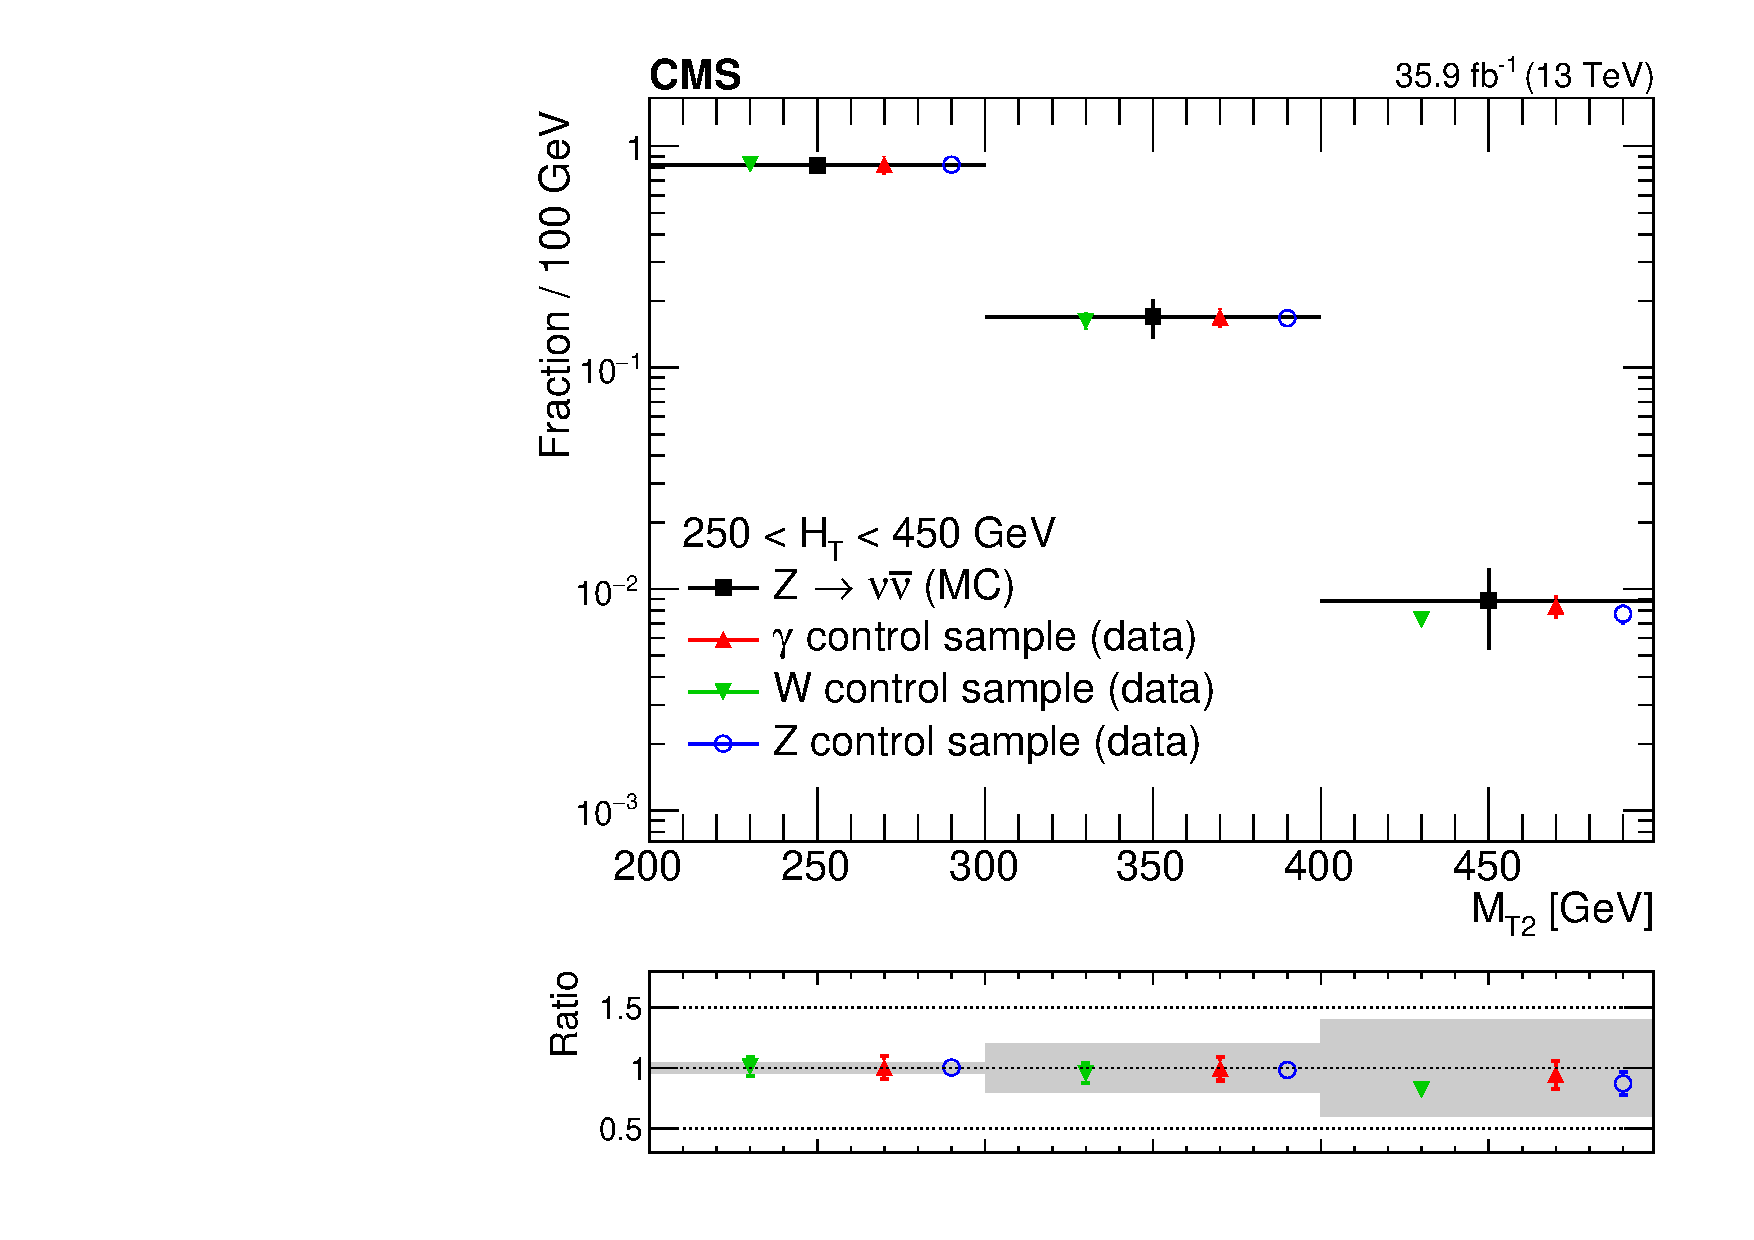
\includegraphics[width=0.4\textwidth]{backgrounds/figs/MT2VL_W_GJ_log}
	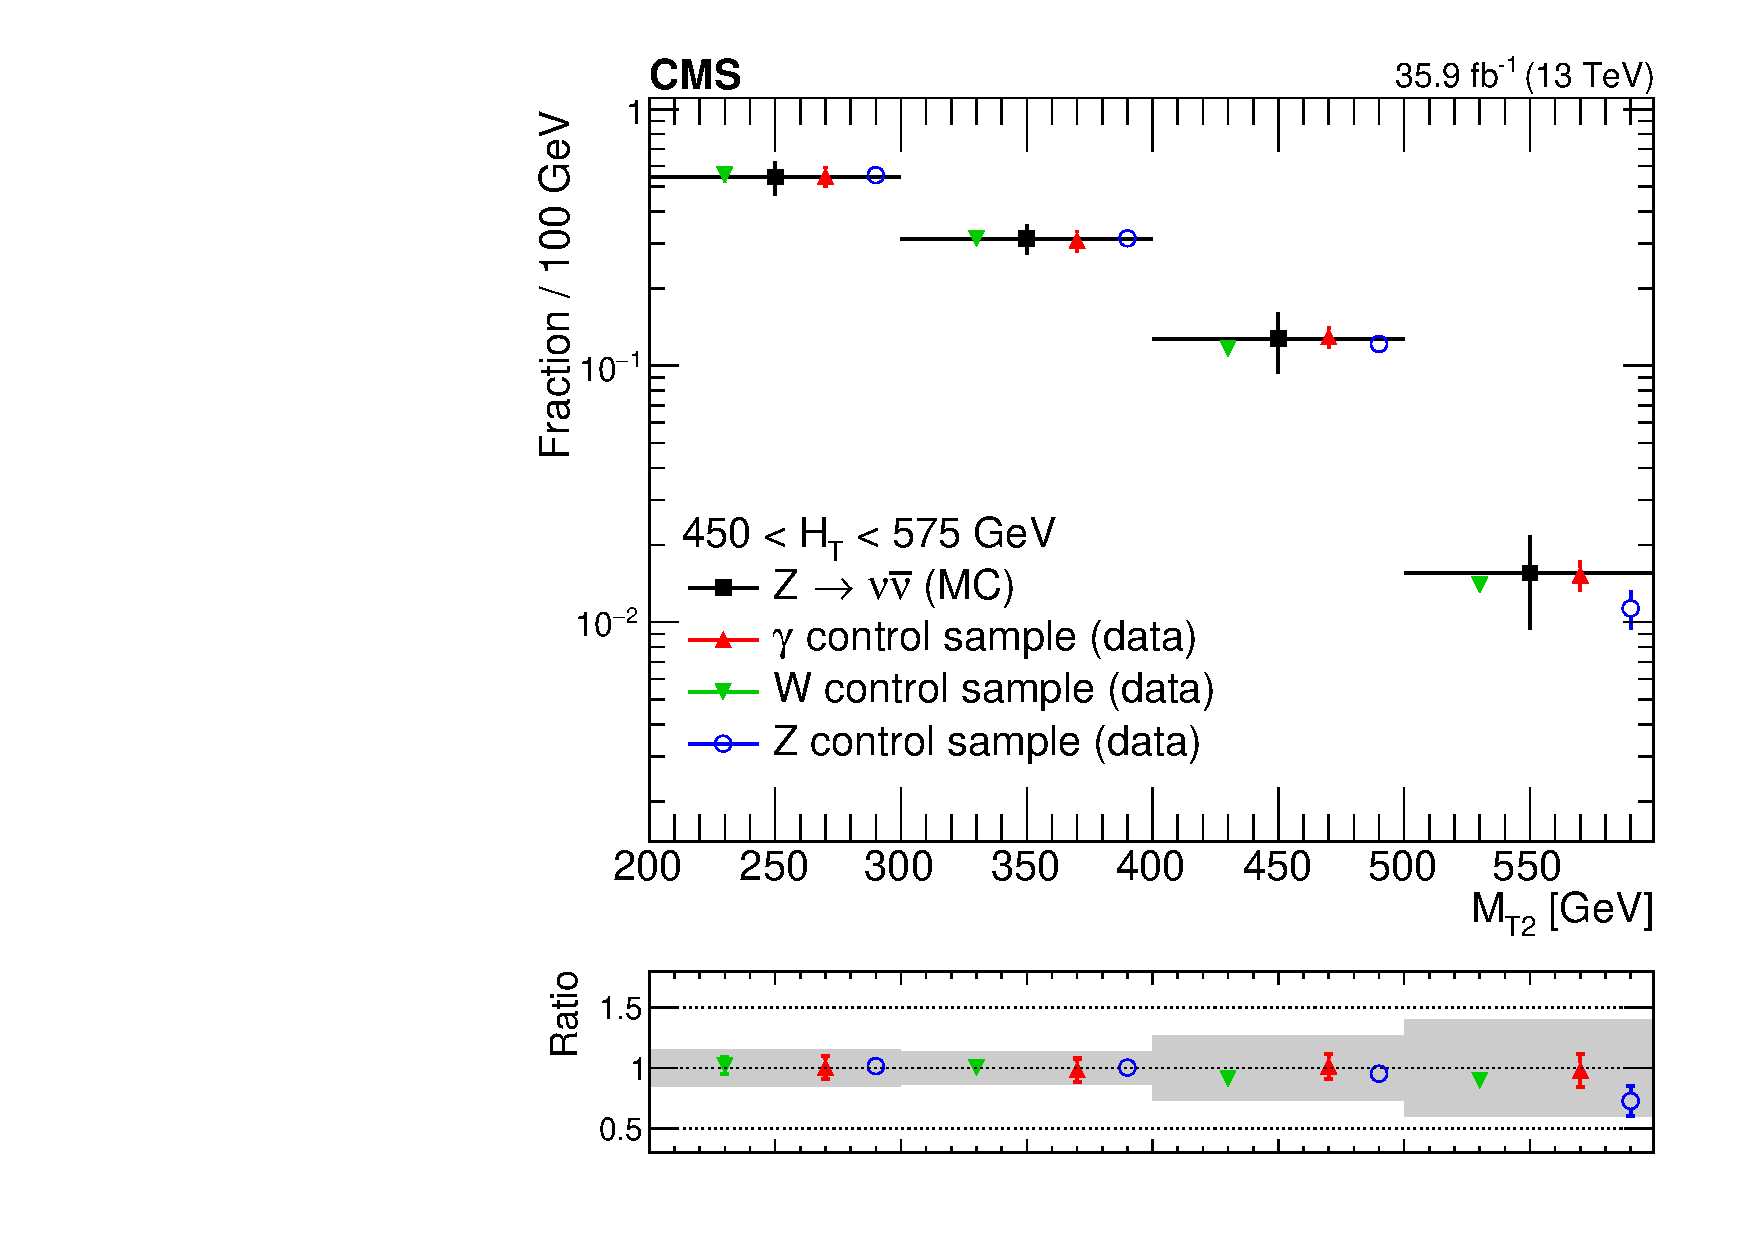
\includegraphics[width=0.4\textwidth]{backgrounds/figs/MT2L_W_GJ_log}
	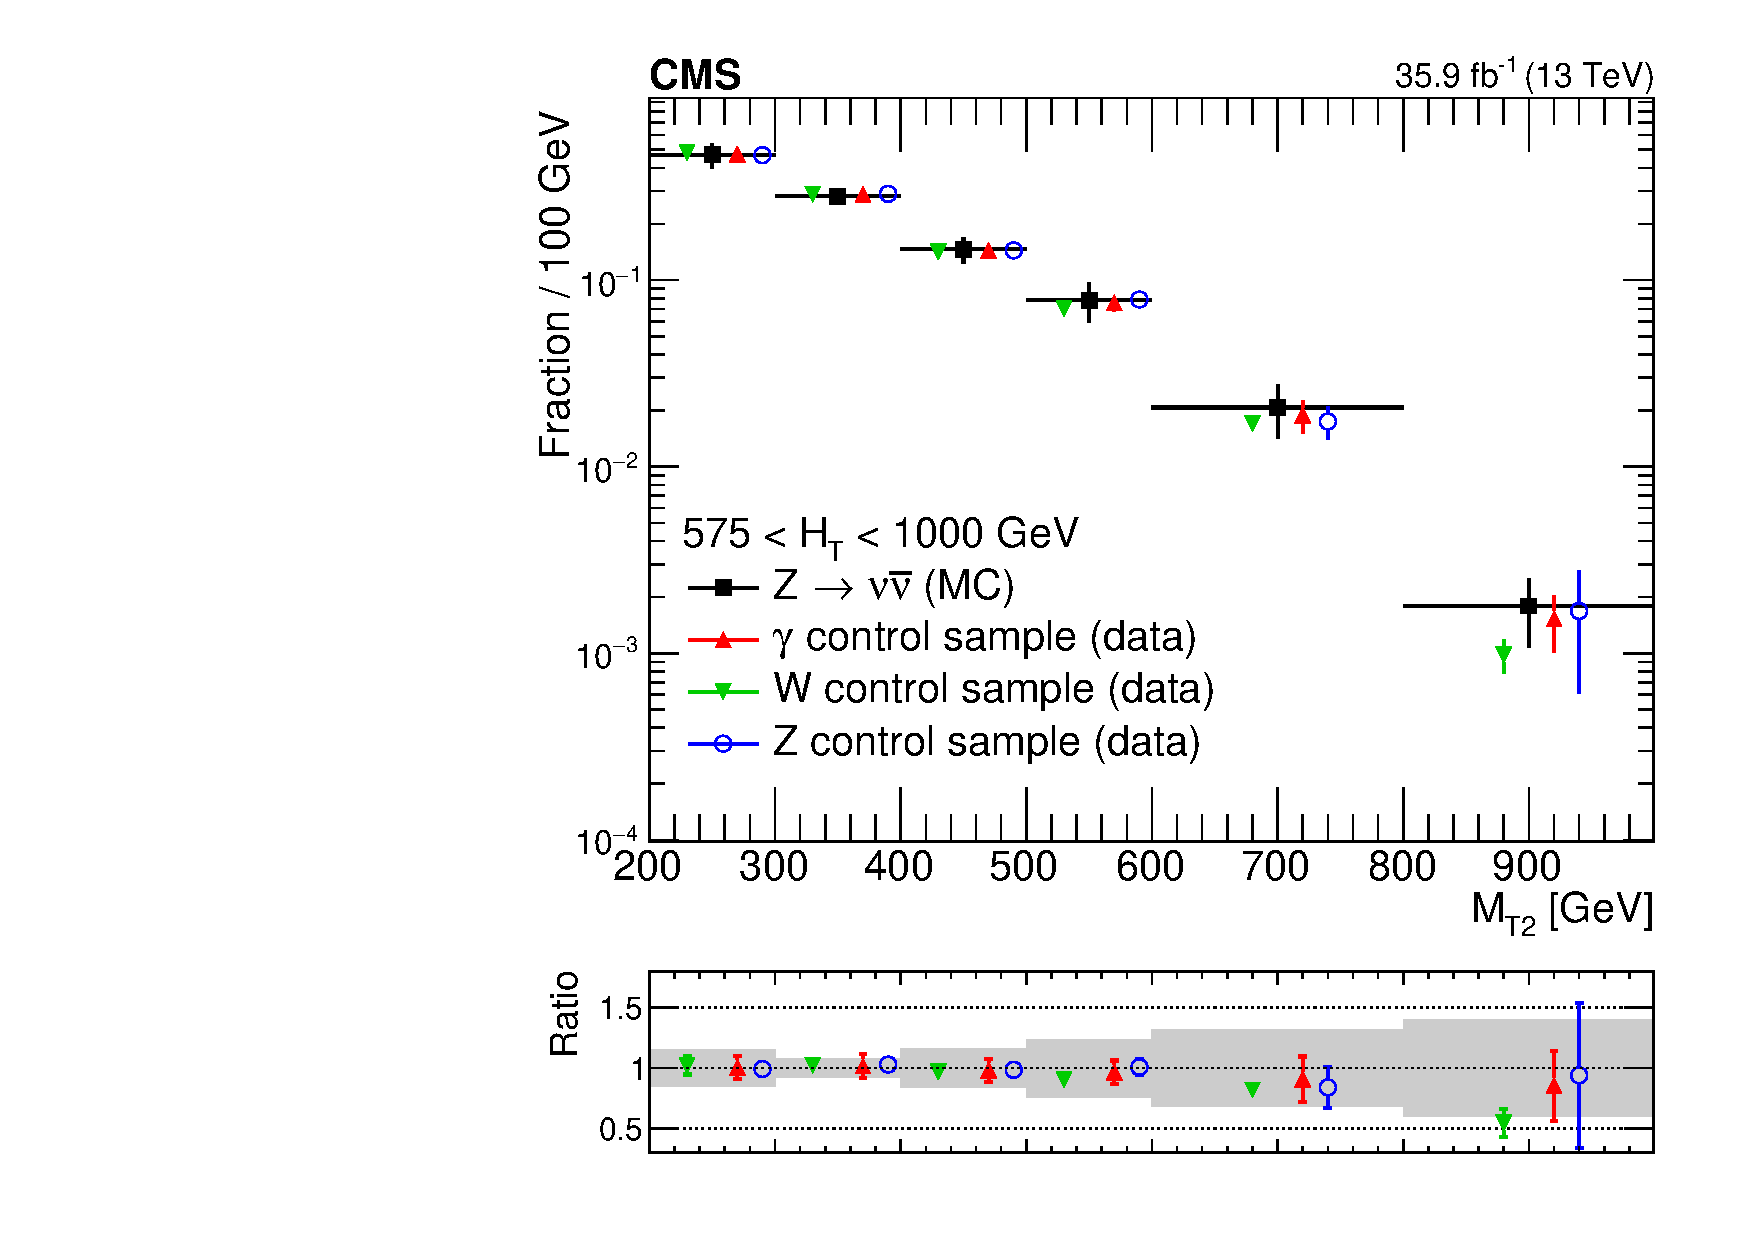
\includegraphics[width=0.4\textwidth]{backgrounds/figs/MT2M_W_GJ_log}
	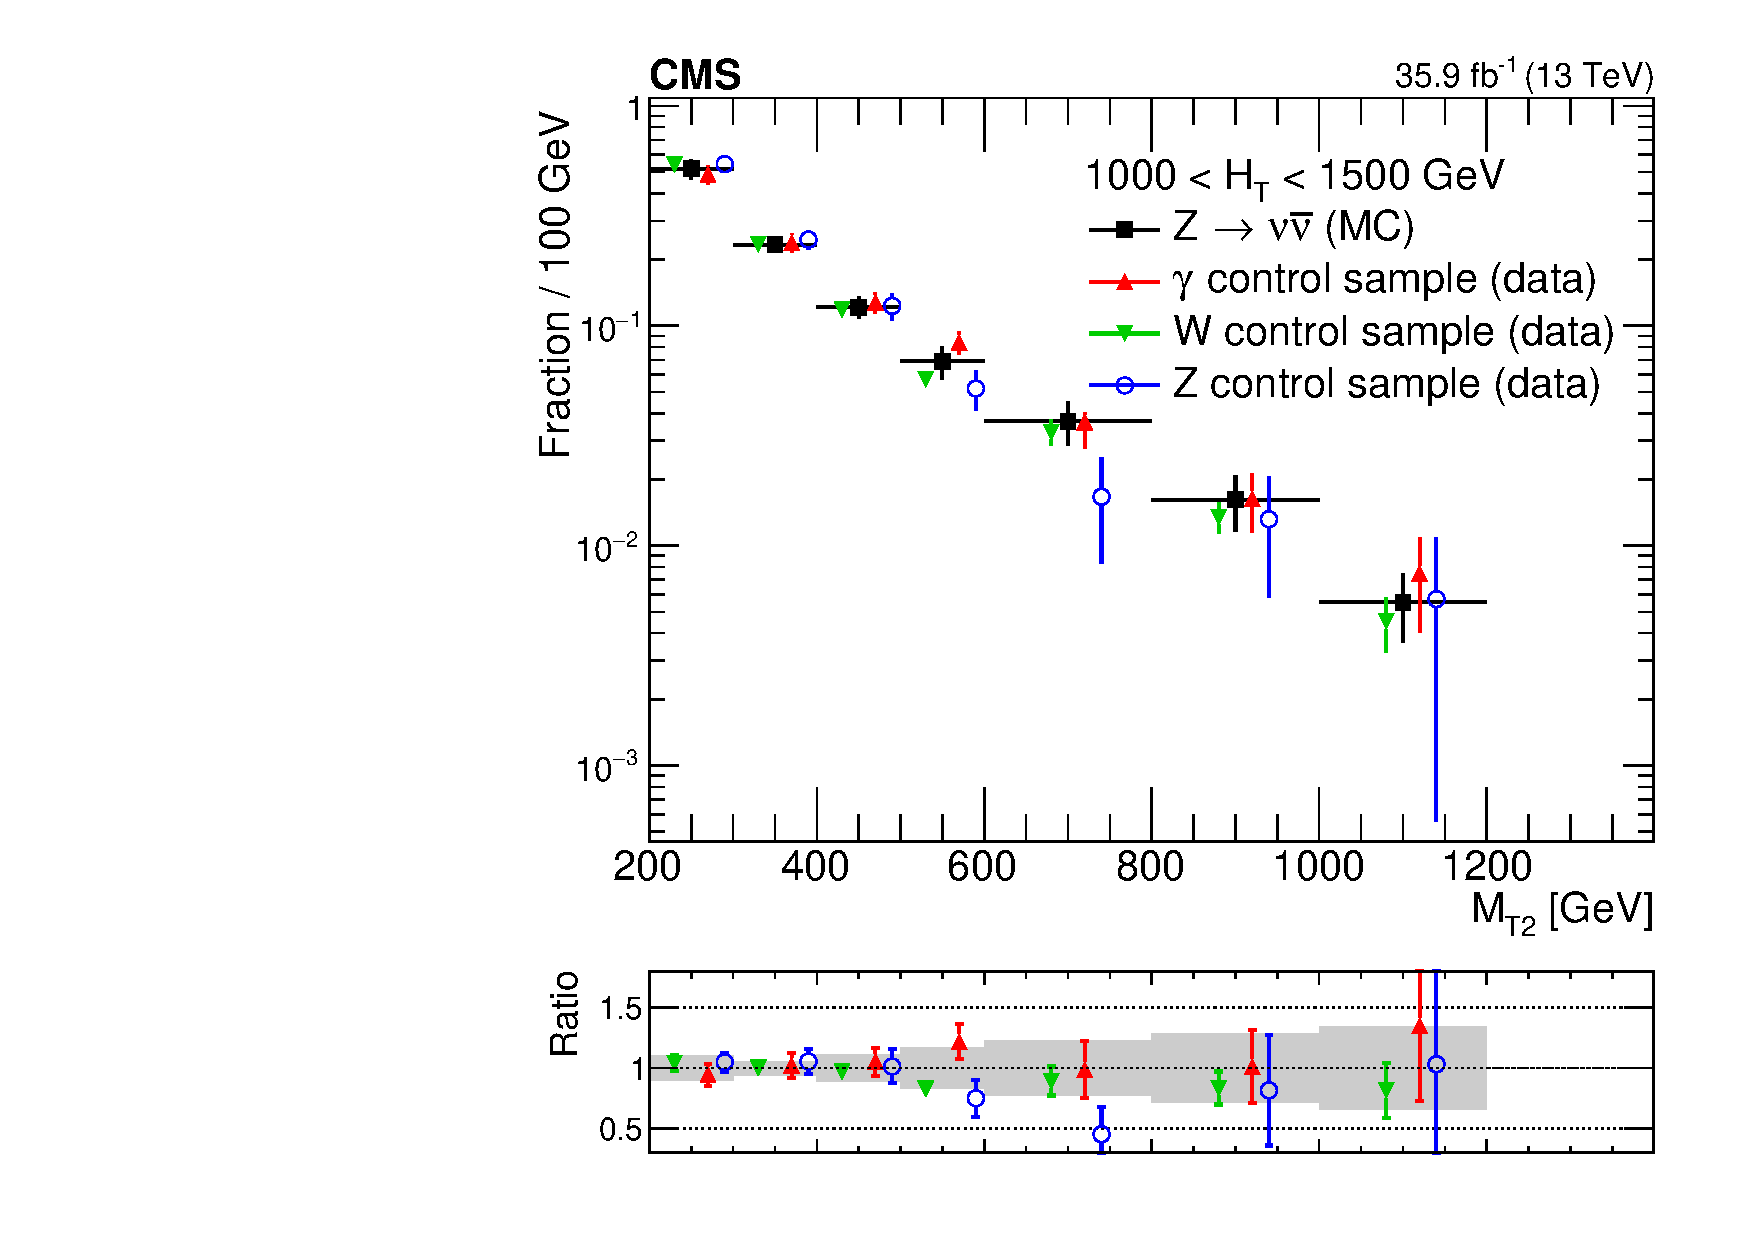
\includegraphics[width=0.4\textwidth]{backgrounds/figs/MT2H_W_GJ_log}
	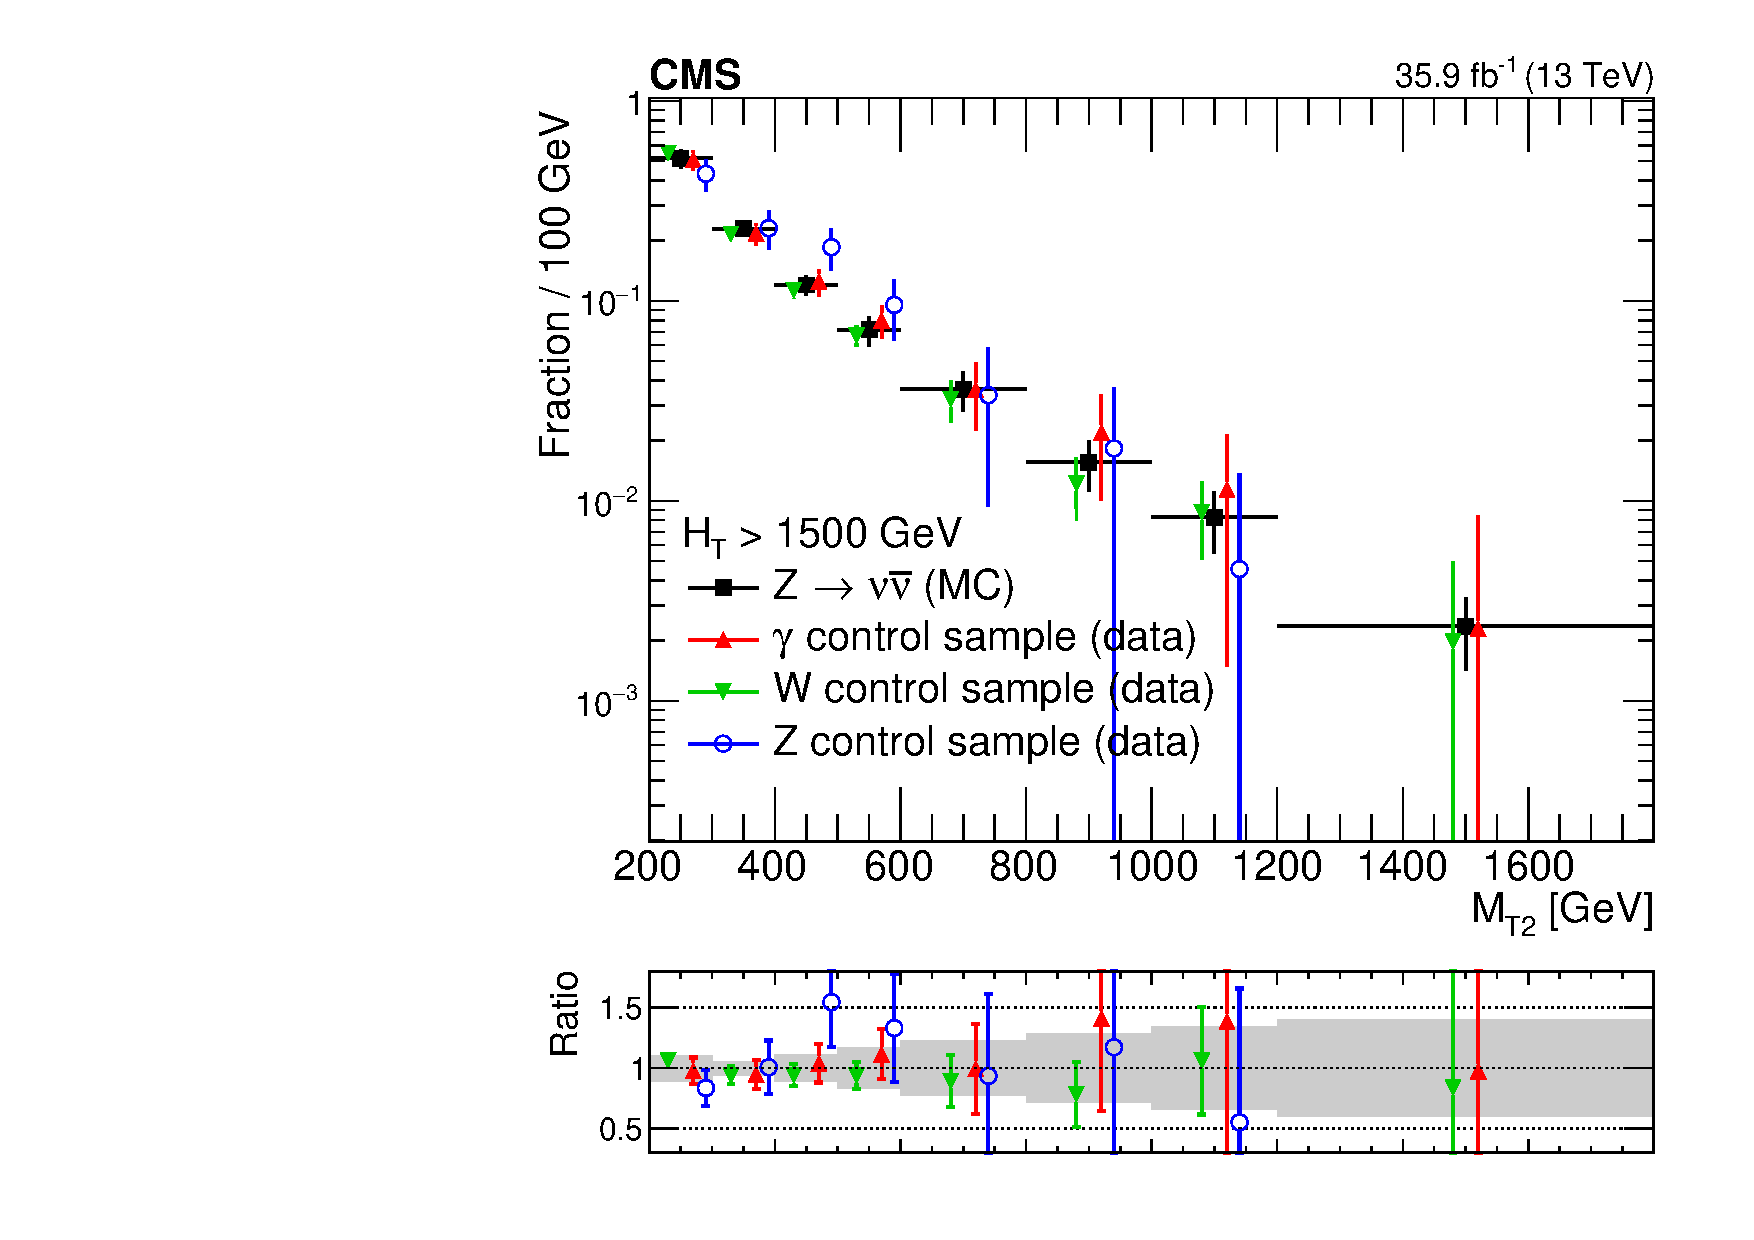
\includegraphics[width=0.4\textwidth]{backgrounds/figs/MT2UH_W_GJ_log}
	\renewcommand{\baselinestretch}{1.0}
	\caption[The \mttwo shape distribution in \znunu simulation compared to $\gamma$, \wlnu, and \zll enriched samples in data, for each \HT region.]{The \mttwo shape distribution in \znunu simulation compared to $\gamma$, \wlnu, and \zll enriched samples in data, for each \HT region. The solid grey band indicates the systematic uncertainty associated with the \mttwo shape modeling.}
	\label{fig:zinvMt2Shape}
\end{figure}

\subsection{Systematic Uncertainties}
\label{subsec:zinvSyst}

Several sources of uncertainty are assessed for the invisible Z estimate, including those associated with the various transfer factors and the \mttwo shape modeling in simulation. The dominant uncertainty in regions using an \mttwo template constructed from data is the statistics of the template. The full list of systematic uncertainties is as follows:
\begin{itemize}
	\item {\it Control region statistical error:} the Poisson error on the number of observed events in \zll data is taken as an uncorrelated uncertainty across all signal regions.
	\item {\it $R_{\mathrm{MC}}^{\znunu/\zll}$ statistical error:} the statistical error associated with the number of MC events generated factors into the transfer factor.
	\item {\it $R_{\mathrm{MC}}^{\znunu/\zll}$ systematic error:} a 5.5\% uncertainty based on variations of lepton efficiency uncertainties as well as other modeling parameters (jet energy scales, factorization and renormalization scales, etc.) is applied as a correlated error in each topological region.
	\item {\it Flavor-symmetric subtraction statistical error:} a Poisson error based on the number of observed opposite-flavor events is assigned to the purity correction.
	\item {\it Flavor-symmetric subtraction systematic error:} a 15\% uncertainty on the \ttbar contamination is taken based on the $R^{\mathrm{SF/OF}}$ uncertainty.
	\item {\it \mttwo shape uncertainty:} in regions where the simulation is used to model the \mttwo distribution, additional variations of the renormalization and factorization scales, parton distribution functions, b-tagging scale factor uncertainties, and jet energy scale uncertainties are performed to measure their effect on the \mttwo shape modeling. The most significant impact is seen in the highest \mttwo bins of up to 20\%. In order to cover the uncertainty from additional electro-weak corrections not present in simulation (and possibly not covered by the above variations), a conservative upper threshold of 40\% is used, and the shape uncertainty (in regions where MC \mttwo shape modeling is used) is assigned as a linear morphing of the \mttwo shape starting in the first bin from which MC extrapolation is used, growing to 40\% in the final bin. The shape morphing in every distinct topological region is taken as an uncorrelated error.
	
\end{itemize}


% --------------------------------------------------------------------------- %
% --------------------------------------------------------------------------- %
